% rubber: module pdftex
% rubber: module index
% rubber: module xr
\documentclass[a4paper,american,12pt]{scrreprt}

\usepackage[margin=1.5cm]{geometry}

\usepackage{graphicx}
\usepackage[headsepline]{scrpage2}
\usepackage[utf8]{inputenc}
\usepackage[T1]{fontenc}
\usepackage{color}
\usepackage{caption}

\usepackage{subcaption}

%\usepackage{times}
%\usepackage{lmodern}
\usepackage{mathptmx}
% required for mathbb
\usepackage{amsmath}
%\usepackage{courier}

\usepackage{txfonts}
%\usepackage[scaled=.9]{helvet}

\usepackage{babel}
\usepackage{microtype}

\usepackage{listings}

\usepackage[hyperfootnotes=false,hidelinks]{hyperref}

\usepackage{todonotes}
\usepackage{xspace}

\usepackage{gitinfo}

\usepackage{tikz}
\usetikzlibrary{shadows}

\automark[section]{chapter}

\parskip.5em
\parindent0em

\newcommand{\cinco}{\textsc{Cinco}\xspace}
\newcommand{\code}[1]{\texttt{#1}}
\newcommand{\key}[1]{\mbox{[#1]}}
\newcommand{\newnotion}[1]{\emph{#1}}
\newcommand{\gui}[1]{\flqq{}\textsf{#1}\frqq{}}
\newcommand{\mgl}[1]{\raisebox{-0.05em}{\mbox{
\includegraphics[height=0.7em]{icons/mgl_icon.pdf}}\kern 0.2em \code{#1}}}
\newcommand{\msl}[1]{\raisebox{-0.05em}{\mbox{
\includegraphics[height=0.7em]{icons/msl_icon.pdf}}\kern 0.2em \code{#1}}}

% Thanks to Thorsten Donig for the nice keystroke visualization
% https://tex.stackexchange.com/questions/5226/keyboard-font-for-latex#5227
\newcommand{\keystroke}[1]{%
  \raisebox{0.15em}{
  \tikz[baseline=(key.base)]
    \node[%
      draw,
      fill=white,
      drop shadow={shadow xshift=0.25ex,shadow yshift=-0.25ex,fill=black,opacity=0.75},
      rectangle,
      rounded corners=2pt,
      inner sep=1pt,
      line width=0.5pt,
      font=\scriptsize\sffamily
    ](key) {\ #1\ \strut}
  ;
  }
  \kern -0.25em
}

\definecolor{numbergray}{gray}{0.5}

\lstdefinestyle{mgl}{
   %language=XML,
   columns=fixed,
	breaklines=true,
	numbers=left,
	numberstyle=\tiny,
	stepnumber=1,
	numbersep=5pt,
   showspaces=false,
   showstringspaces=false,
   frame=tblr,
   tabsize=2,
   frame=shadowbox,
   columns=fixed,
   basicstyle=\ttfamily\scriptsize,
   %basicstyle=\scriptsize,
   rulesepcolor=\color[rgb]{0.6, 0.6, 0.6},
   %keywordstyle=\color[rgb]{0.5,0,0.4}\textbf, 
    keywordstyle=\color[rgb]{0.5,0,0.34}\textbf,
   %keywordstyle=\color[rgb]{0.5,0,0.4}\bfseries, 
   %keywordstyle=\color[rgb]{0.5,0,0.4},
   stringstyle=\color{blue},
   commentstyle=\color[rgb]{0.4,0.7,0.4},
   backgroundcolor=\color[rgb]{0.97,0.97,0.97},
   morekeywords={node, edge, attr, container, as, package, nsURI, iconPath, diagramExtension, graphModel, incomingEdges, outgoingEdges},
	morestring=[b]",
   showtabs=false,
	morecomment=[l]{//},
	morecomment=[s]{/*}{*/},
   literate={0}{{{\color{numbergray}0}}}{1}%
		{1}{{{\color{numbergray}1}}}{1}%
		{2}{{{\color{numbergray}2}}}{1}%
		{3}{{{\color{numbergray}3}}}{1}%
		{4}{{{\color{numbergray}4}}}{1}%
		{5}{{{\color{numbergray}5}}}{1}%
		{6}{{{\color{numbergray}6}}}{1}%
		{7}{{{\color{numbergray}7}}}{1}%
		{8}{{{\color{numbergray}8}}}{1}%
		{9}{{{\color{numbergray}9}}}{1}
}

\newcommand{\includemgl}[3]{\lstinputlisting[style=mgl, float=tb, caption=#2, label=#3, captionpos=b]{#1}}


\lstdefinestyle{style}{
   %language=XML,
   columns=fixed,
	breaklines=true,
	numbers=left,
	numberstyle=\tiny,
	stepnumber=1,
	numbersep=5pt,
   showspaces=false,
   showstringspaces=false,
   frame=tblr,
   tabsize=2,
   frame=shadowbox,
   columns=fixed,
   basicstyle=\ttfamily\scriptsize,
   %basicstyle=\scriptsize,
   rulesepcolor=\color[rgb]{0.6, 0.6, 0.6},
   keywordstyle=\color[rgb]{0.5,0,0.4}\textbf, 
   %keywordstyle=\color[rgb]{0.5,0,0.4}\bfseries, 
   %keywordstyle=\color[rgb]{0.5,0,0.4},
   stringstyle=\color{blue},
   commentstyle=\color[rgb]{0.4,0.7,0.4},
   backgroundcolor=\color[rgb]{0.97,0.97,0.97},
	morekeywords={nodeStyle, edgeStyle, rectangle, ellipse, roundedRectangle,
	text, polyline, size, corner, position, value, color, lineStyle, lineWidth,
	SOLID, DASH, DASHDOT, DASHDOTDOT, DOT, decorator, location, relativeToMid,
	points, appearance, appearanceProvider, background, foreground, relativeTo,
	ARROW, CIRCLE, TRIANGLE, CENTER, MIDDLE, @, extends},
	morestring=[b]",
   showtabs=false,
	morecomment=[l]{//},
	morecomment=[s]{/*}{*/},
   literate={0}{{{\color{numbergray}0}}}{1}%
		{1}{{{\color{numbergray}1}}}{1}%
		{2}{{{\color{numbergray}2}}}{1}%
		{3}{{{\color{numbergray}3}}}{1}%
		{4}{{{\color{numbergray}4}}}{1}%
		{5}{{{\color{numbergray}5}}}{1}%
		{6}{{{\color{numbergray}6}}}{1}%
		{7}{{{\color{numbergray}7}}}{1}%
		{8}{{{\color{numbergray}8}}}{1}%
		{9}{{{\color{numbergray}9}}}{1}
}

\newcommand{\includestyle}[3]{\lstinputlisting[style=style, float=tb, caption=#2, label=#3, captionpos=b]{#1}}


\lstdefinestyle{java}{
   language=Java,
   breaklines=true,
   numbers=left,
   numberstyle=\tiny,
   stepnumber=1,
   numbersep=5pt,
   showspaces=false,
   showstringspaces=false,
   frame=tblr,
   tabsize=2,
   frame=shadowbox,
   columns=fixed,
   %basicstyle=\ttfamily\small,
   basicstyle=\ttfamily\scriptsize,
   rulesepcolor=\color[rgb]{0.6, 0.6, 0.6},
   %keywordstyle=\color[rgb]{0.5,0,0.4}\bfseries, 
   keywordstyle=\color[rgb]{0.5,0,0.4},
   stringstyle=\color{blue},
   commentstyle=\color[rgb]{0.4,0.7,0.4},
   backgroundcolor=\color[rgb]{0.97,0.97,0.97},
   showtabs=false
}

\newcommand{\includejava}[3]{\lstinputlisting[style=java, float=tb, caption=#2, label=#3, captionpos=b]{#1}}


\begin{document}


\chapter{Basics}

\section{About This Document}

This is the technical manual for the ``\cinco SCCE Meta Tooling Suite'' (in
short just \cinco). It is intended to provide a basic usage introduction as
well as (coming soon) reference for all features and keywords. It only implicitely covers the
conceptual ideas behind \cinco. For a more in-depth and scientific view on those,
please refer to the following publications:
%
\begin{itemize}
\item S. Naujokat et al.: Full generation of domain-specific graphical modeling tools: a
meta$^2$modeling approach \cite{NaLSKM2014}
\item S. Naujokat et al.: Domain-Specific Code Generator Modeling: A Case Study for
Multi-Faceted Concurrent Systems \cite{NaTISL2014}
\item D. Kopetzki: Model-based generation of graphical editors on
the basis of abstract meta-model specifications \cite{Kopetz2014}
\end{itemize}

This document will constantly be revised and extendend. The latest version will
always be available for download at \url{http://cinco.scce.info}. 

\begin{description}
\item[covered version] \cinco v. 0.5
\item[git commit id] \gitAbbrevHash{}
\item[date of build] \today
\end{description}

\section{Introduction}

The ``\cinco{} SCCE Meta Tooling Suite'' is an integrated devlopment environment
(IDE) for the quick and easy development of domain-specific graphical modeling
tools. \cinco{} makes use of several frameworks from the Eclipse Modeling
Project, but its main goal is to hide those frameworks' intricacy from the
tool developer. \cinco{} provides two simple textual specification languages (MGL and
MSL, see below) for the high-level characterization of the developed tool's
structural and visual features. Above that, \cinco{} is also a full Java IDE, so
that the portions of the developed tool that are not described in a declarative
way can seamlessly be developed in the same environment.

Crucial to \cinco is the concept of code generation. Much of the code of a
modeling tool that is developed with \cinco (in the following called \cinco
Product, or just CP) is generated automatically from abstract specifications,
such as the already mentioned MGL and MSL files. It is of utmost importance
that you \emph{never} make any changes to automatically generated
code\footnotemark{}, as all those changes will be gone once the code generation
is run again.

\footnotetext{Of course, this does not apply to automatically generated 'source'
files (such as examples and templates). Those are generated for convenience to
have a basic version to start working on.}

\section{Download \& Installation}

As \cinco{} is a full Eclipse-based IDE including the Eclipse Modeling Tools
(EMF, Xtext, Graphiti, etc.) and the Java Development Tooling (JDT) in addition
to our own plug-ins the download size is almost 300 MB. We are planning to
provide the \cinco{}-specific plug-ins via an Eclipse update site in the future,
but for now you need to download the whole package as one.

Please note: \cinco{} itself is developed under the ``Eclipse Public License v. 1.0'', 
but the executable build contains several libraries from the jABC
project, for which the following license applies:

\begin{verbatim}
===============================================================================
This software is free to use.

You are not allowed to redistribute, modify or decompile this software.

Third-party components are included for which these restrictions may not apply.
Please refer to the documentation for details.

THIS SOFTWARE IS PROVIDED ``AS IS'' AND WITHOUT ANY EXPRESS OR IMPLIED
WARRANTIES, INCLUDING, WITHOUT LIMITATION, THE IMPLIED WARRANTIES OF
MERCHANTIBILITY AND FITNESS FOR A PARTICULAR PURPOSE.
===============================================================================
\end{verbatim}

\cinco{} requires OpenJDK 7 to be installed on your system as main Java
installation (i.e. JAVA\_HOME pointing there). Apart from that, you just have to
choose the correct zip file for download (Linux/Window/Mac in 32 or 64 bit
variant), unzip it and execute the included binary: \code{cinco} for Mac and
Linux, \code{cinco.exe} for Windows.

\section{Getting Started Tutorial}

\subsection{Launching \cinco for the First Time}
\label{sec:firstLaunch}

When launching \cinco{} it will first query you for the location of a workspace
directory. Choose some place on your harddisk that is not within the \cinco
installation folder. This workspace will contain all your \cinco projects
and the according metadata, as well as sub-projects, specification files, source
code etc. It is possible to use different workspaces (e.g. for different
projects). If you don't want to use multiple ones for now, you can check
\gui{Use this as default and do not ask again} before clicking \gui{OK}.

\begin{figure}
	\centering
	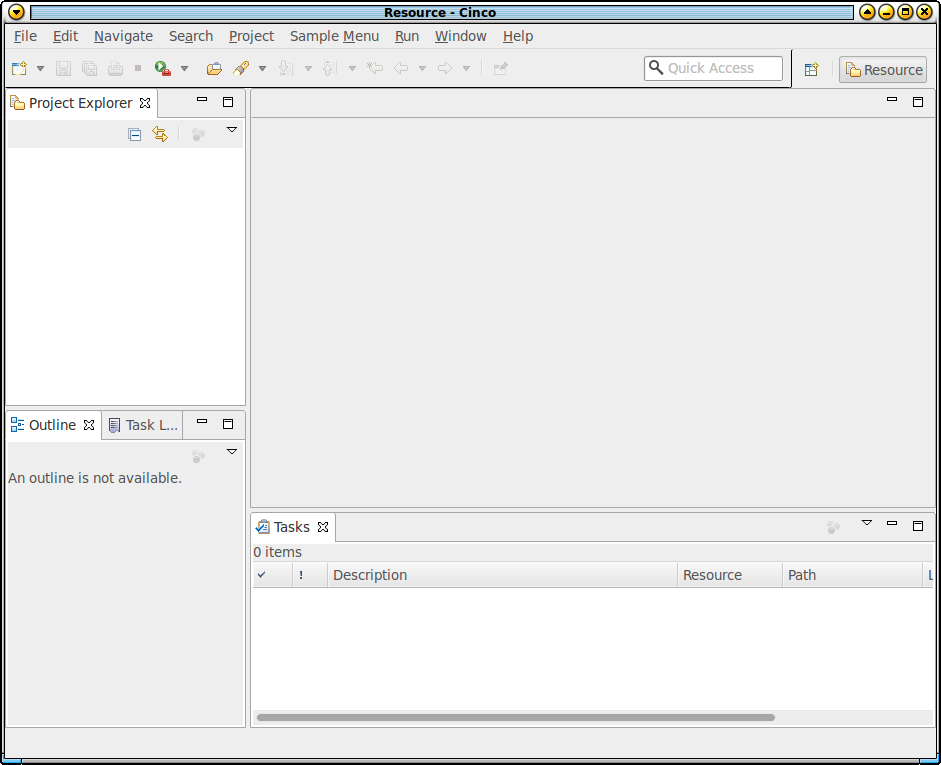
\includegraphics[width=.7\textwidth]{screenshots/cinco-gui-firststart.png} 
	\caption{First startup should look like this}
	\label{fig:firstStart}
\end{figure}

After choosing the workspace \cinco should start and look like
Fig.~\ref{fig:firstStart}. The GUI is partitioned into so-called
\newnotion{Views}. For now, the \gui{Project Explorer} and the editor area (the
big empty grey space on the right) are the most important ones. 

\subsection{Creating a \cinco Product Project}

\begin{figure}
	\centering
	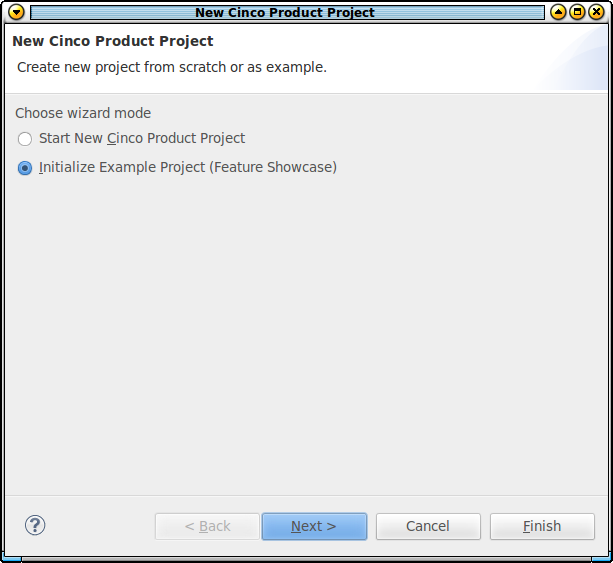
\includegraphics[width=.5\textwidth]{screenshots/new-cp-wizard.png}
	\caption{Use the wizard to create a new example project}
	\label{fig:cpWizard}
\end{figure}

To get a new \newnotion{Cinco Product} project initialized, we'll now use the
built-in wizard to create some example files to start working with.
Right-click somewhere within the \gui{Project Explorer} and choose \gui{New / Cinco Product
Project}. The wizard as depicted in Fig.~\ref{fig:cpWizard} appears. The wizard
has two modes. You can either start a completely new project from scratch or
generate an example project showing off some of the Cinco features. We'll go for
the latter one for now. Select \gui{Initialize Example Project (Feature
Showcase)} and hit \gui{Next}. 

\begin{figure}
	\centering
	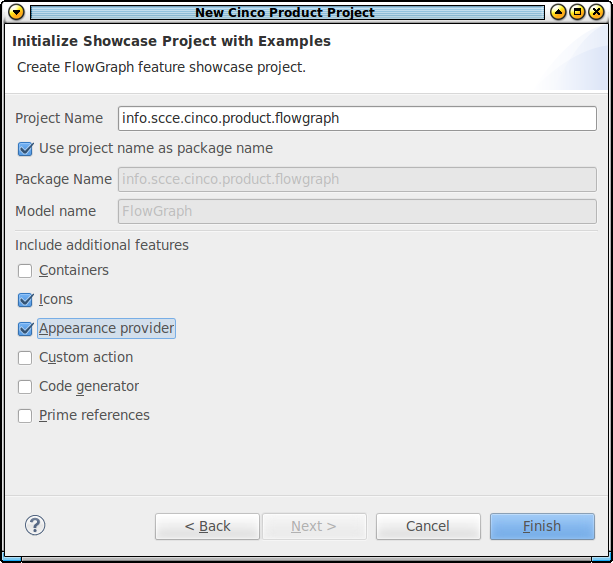
\includegraphics[width=.5\textwidth]{screenshots/new-cp-wizard2.png}
	\caption{Select example features that shall be generated}
	\label{fig:cpWizard2}
\end{figure}

The next page of the wizard now lets you configure some basic things for your
example project (cf. Fig.~\ref{fig:cpWizard2}). Please note that the model name
is fixed, as the generated example is a flow graph. For now, you probably should leave
the project/package name as suggested; if you create additional examples with
the wizard later, you can choose different names here to distinguish them. Each
feature you select at the bottom will generate additional parts in the example.
We suggest to use \gui{Icons} and \gui{Appearance provider} to keep the files
manageable small for your first attempt in using \cinco{}. Confirm your
selection with \gui{Finish}

\begin{figure}
	\centering
	\begin{subfigure}[t]{0.40\textwidth}
		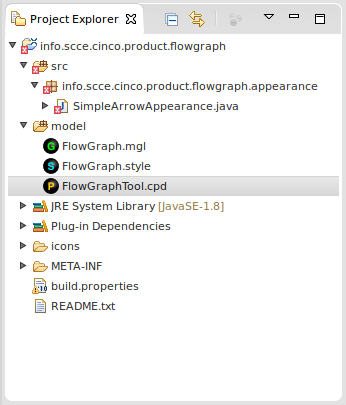
\includegraphics[width=\textwidth]{screenshots/example-cp-pregen.png}
		\caption{Project after running the wizard}
		\label{fig:cpPreGen}
	\end{subfigure}
	\qquad
	\begin{subfigure}[t]{0.40\textwidth}
		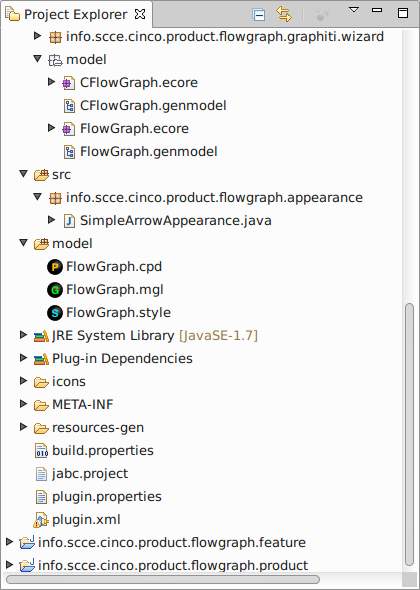
\includegraphics[width=\textwidth]{screenshots/example-cp-postgen.png}
		\caption{Project after code generation}
		\label{fig:cpPostGen}
	\end{subfigure}
	\caption{Project file system view before and after \cinco{} product generation}
\end{figure}

After running the wizard, the project explorer contains your freshly created
project. Depending on the names you've chosen, it should now look somewhat
similar to Fig.~\ref{fig:cpPreGen}. Please note that the compile error marked at
\code{SimpleArrowAppearance.java} is not unexpected. The Java class refers to
other Java entities that have not yet been generated. 

You might want to take a short look into those initialized files (especially the ones in the
\code{model} folder), but before we delve more deeply
into their contents (which we will do
in Sec.~\ref{sec:examplefiles}), let's first generate this example CP and give
it a try. Just right-click on the \mgl{FlowGraph.mgl} and
choose \gui{Generate Cinco Product}. Shortly after, your project explorer should
look like Fig.~\ref{fig:cpPostGen}. Several new files, directories and a new
project -- which will be even more than one once you start using advanced
features of \cinco{}, such as meta plug-ins -- have been generated. Also, the
compile error we've noticed before is gone. 

Whenever you change the CP's specification files, you need to re-generate the
code. Sometimes you also need to delete all the generated code, e.g. when
deleting or renaming a node type. But as you never do any manual changes to the
generated code, this is no problem. 

\subsection{Testing the \cinco Product}

Now, let's test the tool we just generated. Within the project explorer,
right-click on the root folder of your main project and choose \gui{Run As /
Eclipse Application}. You should now see the \cinco splash screen again,
starting a different Eclipse product: your modeling tool. \footnotemark

\footnotetext{Please note: When you use the here presented 'simple way' of
starting your product (via the \gui{Run As} menu) you will actually start your
tool including \emph{all} the \cinco plug-ins and libraries. In fact, you start
a second \cinco enriched with the new features we just generated. This is
ususally not what is desired, because a tool developer needs to work with different tools
than the tool user. The advanced topic of own product definitions with a minimal
required set of plug-ins will be added to this manual later. We even plan
eventually provide automization for this task. For testing purposes, however,
this does not impose any problems other than ample unnecessary GUI elements.}

Again, you should see an empty tool like Fig.~\ref{fig:firstStart}. To create a
new model we first need a new project where it can be placed. This time,
however, we don't need a \cinco product project (as we don't want to develop
another \cinco product within the just started \cinco product). A plain project
is enough this time. Right-click somewhere in the project explorer and select
\gui{New / Project... / General / Project / Next >}, give the project some name
and click \gui{Finish}. Then, right-click on your newly created project and
select \gui{New / Other... / Cinco Product / New FlowGraph} to create your
first CP-specific model.

The editor area now shows your empty model with a drawing grid. On the right
side you see a \gui{Palette}, containing the elements you can now use for modeling.
The elements you see there are in the \gui{Palette / Objects}
category: \code{Start}, \code{End}, and \code{Activity}. Those are the three node
types that are were automatically included in the \mgl{FlowGraph.mgl} by the
wizard. Begin modeling by just drag\&dropping a few different nodes into the
modeling area. To connect nodes, you can just hover over a node and drag the small
appearing arrow icon onto a target node. For the \code{Activity} node type and
the edges originating from them, you can use the \gui{Properties} view (bottom
of your window) to set attributes; \code{Name} and \code{Description} for the
node as well as \code{Label} for the edge. An activity's name is displayed
within the node shape (the blue box) and the edge label is shown as a floating
(and movable) textbox next to the edge. Fig.~\ref{fig:firstModel} shows an
example how your tool should look now.

\begin{figure}
	\centering
	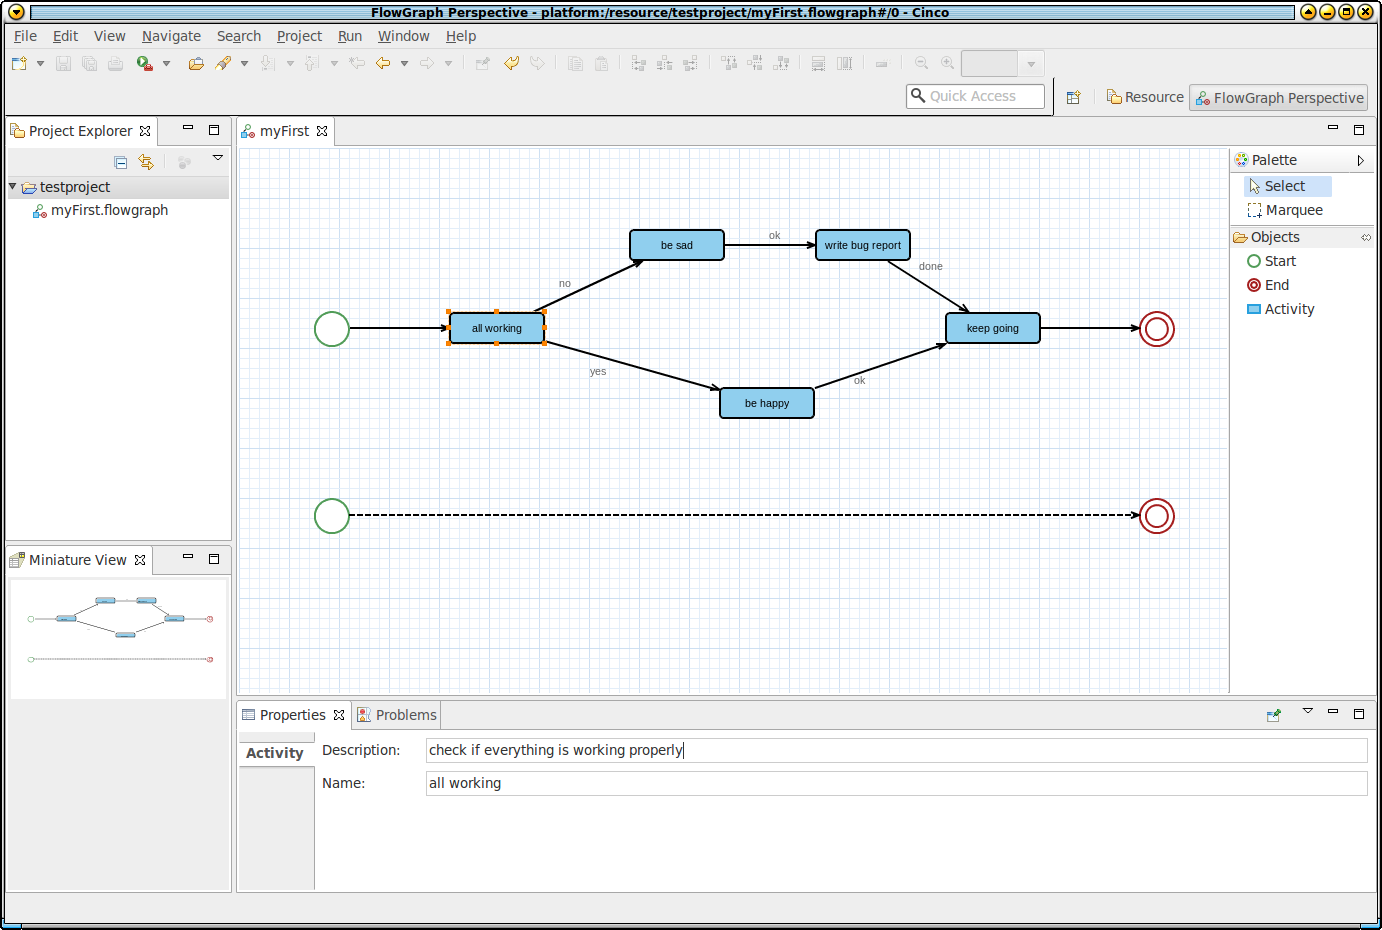
\includegraphics[width=.9\textwidth]{screenshots/cp-first-model.png} 
	\caption{The first model that was modeled using the example \cinco product}
	\label{fig:firstModel}
\end{figure}

The modeling elements abide by the following syntactic rules:

\begin{itemize}
\item \code{Start} nodes (green circle) have at most one outgoing edge of type
	\code{Transition}, but no incoming edges.
\item \code{End} nodes (double red circle) have arbitrarily many incoming edges,
	but no outgoing.
\item \code{Inner} (blue box) nodes have multiple outgoing edges of type
	\code{LabeledTransition}, and may have multiple incoming edges of both types.
	The attribute \code{Text} is displayed centered within the box.
\item \code{LabeledTransition} edges connect \code{Inner} nodes with others and
	have their attribute \code{Label} displayed as movable caption next to it.
\item \code{Transition} edges only originate from \code{Start} nodes. If such an
	edge directly leads to an \code{End} node, it is displayed with a dashed
	line.
\end{itemize}

Those rules are all defined within the example \cinco specification files that
were created by the wizard. The next section will therefore provide a detailed
discussion on the contents of those files.

\section{Discussion on the Example Files}
\label{sec:examplefiles}

We consider our specification formats MGL and MSL fairly self-explanatory,
meaning that one usually can understand most of their contents without detailed
knowledge on available keywords or syntactic structures. This section
will nonetheless detail on our two example files, but you might want to have a look at
your \mgl{MyModelType.mgl} and \msl{MyModelType.style} beforehand, to decide for
yourself. 

However, writing a programming or specification language usually is a totally
different matter. But here, \cinco heavily benefits from it being implemented
with libraries from the Eclipse Modeling Project, in this case especially Xtext:
The so-called \newnotion{Content Assist} that is generated for every Xtext-based
editor provides a very useful autocompletion when
\keystroke{Ctrl}+\keystroke{Space} is pressed (if you ever programmed Java using
Eclipse, you most likely know this shortcut already). With this feature it is
often not even required to read the documentation, as one can autocomplete
through the whole specification file, manually inserting an identifier every now and
then.

Modeling tool development with \cinco centers around two textual specification
files. On the one hand we have a file in the ``Meta Graph Language'' (MGL) that
contains the structural information on the tool's model. On the other hand, a
``Meta Style Language'' (MSL) file\footnotemark{} is required to specify the
visual characteristics (e.g.  shapes and colors) of this model. The following
subsections will each provide an introduction to one of this specification
languages alongside the example files created by the new project wizard.

\footnotetext{Please note that the file extension for MSL is currently
\code{.style}. We are planning to change this to \code{.msl} in a future
release.}


\subsection{MGL File}

\includemgl{listings/MyModelType.mgl}{Example MGL file}{lst:myMGL}

Listing \ref{lst:myMGL} shows the \mgl{MyModelType.mgl} as it was initialized in
Sec.~\ref{sec:firstLaunch}. Aside from some general configuration stuff in lines
1-5, it contains two different kinds of entitiy declaration:
\begin{enumerate}
\item Node type declarations
\item Edge type declarations
\end{enumerate}

\subsection{MSL File}

\includestyle{listings/MyModelType.style}{Example MSL file}{lst:myMSL}


%\chapter{Advanced Topics}

%\section{Containers Types}
%\section{Prime References}
%\section{Custom Features}
%\section{Code Generation}
%
%\chapter{Language Reference}
%
%\section{Meta Graph Language (MGL)}
%\section{Meta Style Language (MSL)}
%\section{Annotations}


\bibliographystyle{alpha}
\bibliography{world}


\end{document}
